%- - - - - - - - - - - - - - - - - - - - - - - - - - - - - - - - - - - -
%- - - - - - - - - - - - - - - - - - - - - - - - - - - - - - - - - - - -
%  QPLIB-3.tex
%- - - - - - - - - - - - - - - - - - - - - - - - - - - - - - - - - - - -
%- - - - - - - - - - - - - - - - - - - - - - - - - - - - - - - - - - - -
\section{Library Construction}\label{sec:lib}

In this section we present all the steps performed in order to build
the library. In particular we describe the first set of gathered
instances (Section \ref{subsec:instColl}),
we present the feature used to classified the instances (Section
\ref{subsec:feature}),
we discuss the issues concerning the format of the instances (Section
\ref{subsec:format}),  and finally we describe the selection process
used to filter the instances in order to construct the final library
(Section \ref{subsec:selection}).

%- - - - - - - - - - - - - - - - - - - - - - - - - - - - - - - - - - - -
\subsection{Instance Collection}\label{subsec:instColl}

In this section we describe the procedure we adopted to gather the
instances. In January $2014$, we issued an online call for instances
using the principal international mailing lists.
In particular, we addressed the mailing lists of the mathematical
optimization and numerical analysis communities, reaching in this way
the largest possible set of interested researchers and practitioners.
The call remained open for 10 months, during which we received a large
number of contributions with different characteristics. The instances
we received  comes from theoretical studies and from real-world
applications.

In addition to spontaneous contribution we analysed the other generic
libraries of instances available  on internet and containing quadratic
instances. Namely, we cite here the libraries from which we selected
some quadratic instances:

\begin{itemize}
 \item {\tt BARON Library}
\url{http://www.minlp.com/nlp-and-minlp-test-problems}
 \item {\tt CUTEst Library}
\url{https://ccpforge.cse.rl.ac.uk/gf/project/cutest/wiki}
 \item {\tt GAMS Library}
\url{http://www.gamsworld.org/performance/performlib.htm}
 \item {\tt MacMINLP} \url{https://wiki.mcs.anl.gov/leyffer/index.php/MacMINLP}
 \item {\tt Meszaros} \url{http://www.doc.ic.ac.uk/~im/00README.QP}
 \item {\tt MINLP} \url{http://www.gamsworld.org/minlp/minlplib.htm}
 \item {\tt POLIP} \url{http://polip.zib.de/pipformat.php}
\end{itemize}

Other quadratic instances were found in online libraries devoted to
specific optimization problems that can be modelled as quadratic ones:
Max-Cut, Quadratic Assignment, Portfolio Optimization and several
others.

At the end of this process we gathered more than eight thousand
instances. Three fourths of them contained discrete variables, while
the remaining ones contained only continuous variables.

More in details, we gathered a large number of Quadratic Binary Linear
(QBL), Quadratic Continuous Quadratic (QCQ) and Quadratic General
Quadratic (QGQ) instances, i.e., $\approx 1800$ instances, $\approx
2000$ instances and $\approx 2500$ instances respectively.
We gathered $\approx 1000$ Convex General Convex (CGC) instances. We
gathered relatively few Quadratic Binary Quadratic (QBQ), Convex
Continuous Convex (CCC) and Convex Mixed Convex (CMC) instances, i.e.,
$\approx 150$ instances, $\approx 200$ instances and $\approx 200$
instances respectively. Finally we gathered only $17$ Quadratic Mixed
Linear (QML) instances.

In the call for instances no specific formats were imposed
%we did not impose a specific format
for the submissions.
%In this phase we also eliminated multiples copies of the same instance.
To evaluate the instances we decided, for practical reasons, to use
Gams as common platform for all the experiments involving commercial
solvers.
For this reason, we decided to translate all instances into the
\texttt{.gms} Gams format and \texttt{.lp} format.
 In a preliminary phase, all the instances received were divided
according to their format and subsequently translated.
%In \S~\ref{subsec:tools}
%%~\ref{subsec:CP_convex}
%the tools used
%to translate an instance from a given format to the \texttt{.gms} format
%%to translate an instance from and to a given format to the
\texttt{.gms} format
%are described in more detail.\\

In addition, we have introduced
a specific format \texttt{.qplib}. This new format is capable of describing
all the instances of the library in a sparse form.
In comparison to a more \emph{high level} format like \texttt{.gms}, the new
format presents two advantages:
it is easier to read by a self-made parser and it produces smaller files.
See Appendix~\label{sec:format} for details.
%\textcolor{red}{ToDo: describe \texttt{.qplib} format. Maybe in an appendix?}

% is lighter in terms of sie
%  significantly
%less memory
%in comparison and

% for this reason we used the \texttt{.gms} format as one of the
format of the library. %checked if one instance was present copies of
the same instance, potentially written in different formats



\subsection{Instance Features}\label{subsec:feature}

For each instance of the starting set, we collected the following
characteristics which allow to classify the instances into the
categories described in Section~\ref{sec:QPbasic}.


As far as the variable type is concerned, we gather the following information:
\begin{itemize}
\item number of binary variables (\emph{\# bin}),
\item number of integer variables (\emph{\# int}),
\item number of continuous variables (\emph{\# cont}).
\end{itemize}
In case at least one binary or integer variable is present, then the
instance is categorized as \emph{discrete} instance, on the other
hand, in case only continuous variables are presents, the instance is
categorized as \emph{continuous}.

As fas as the objective function is concerned, we gathered the
following information:
\begin{itemize}
\item Percentage of negative eigenvalues (\emph{\% neg eig}),
\item Density of the Hessian of the objective function (\emph{\% dens}).
\end{itemize}
 The number of negative eigenvalues of the Hessian matrix allows to
identify the specific objective function type, i.e. in presence of at
least one negative eigenvalue, the objective function is non convex.
The density of the Hessian of the objective function is defined as the
number of nonzero entries     over the total possible figure.

As far as the constraint type is concerned, we gather the following information:
\begin{itemize}
\item number of linear constraints (\emph{\# lin}),
\item number of quadratic constraints (\emph{\# quad}),
\item number of convex constraints (\emph{\# conv}),
\item number of box constraints (\emph{\# box}).
\end{itemize}
A constraint is considered quadratic if it contain a quadratic term.
Among the quadratic constraints, the one with only non negative
eigenvalues are classified as convex constraints.

This information allows to have a static picture of the main features
of the instances.


\subsection{Instance Selection}\label{subsec:selection}

The first goal of the library is to gather ``challenging'' instances,
i.e., instances which can not be easily solved by the state of the art
solvers.
The second goal of the library is to represent the largest majority of
the different categories of quadratic problems.
The third goal is to include in each of the categories a set of well
diversified instances.
Finally, the fourth goal is to obtain a library whose set of instances
is neither too small either too large, to preserve statistical
relevance while at the same time being computationally manageable.

To achieve the aforementioned goals, we performed the following two
filters applied in cascade.

\begin{itemize}
\item \emph{First Instances Filter.}\\
The first filter is design to drastically reduce the number of
instances by eliminating the easy instances. An empirical measure way
of testing the hardness of an instance is the CPU time needed by a
complete solver (cf.~\S \ref{sec:algo}) to solve the instance to
global optimality.
In this step, we decided to use the broadest set of solvers able to
tackle the different categories of quadratic problems.\\
Accordingly, for each of the gathered instance, we run the solvers in
{\tt Gams} (see Table \ref{}) able to solve it to global optimality.
The number of solvers depends on the category of the instances under
consideration.
We the filtered according to a relative measure of computational
difficulty, i.e., we discarded all instances that are solved by at
least 30\% of the complete solvers within a time limit of 30 seconds.
\item \emph{Second Instances Filter.}\\
The goal of the second filter is to eliminate instances that are similar.
We used the instance features presented in
Section~\ref{subsec:feature} and the CPU solving time obtained in the
first filter to guide this second step. \\
We carefully analysed the instances and we grouped them accordingly to
similar features and CPU time. To reduce the size of the test-bed
while keeping the representativeness of the library,     we kept for
each cluster of similar instances one representative.\\
In order to have a deeper insight on the computational hardness of the
instances we performed a second round of tests on the resulting set of
instances.  We used a general purpose solverand we set the time limit
to 120 seconds. Finally, all the instances which have been solved to
proven optimality have been discarded.
\end{itemize}
In Table~\ref{tab:filters} we summarize the two filter steps, which
allows us to identify the final set of $251$ discrete instances and
$116$ continuous instances.








\begin{center}
\begin{table}[]
 \centering

 \setlength{\tabcolsep}{5pt}
%  \arraystretch{1}
\begin{tabular}{cccc}
Starting set& \multicolumn{ 2}{c}{ $\approx$ 8500 Instances }& \\
& \multicolumn{ 2}{c}{$\Downarrow$}& \\
& $\approx$ 6000 Discr. Inst.  & $\approx$ 2500 Cont. inst. & \\
First Filter  & $\Downarrow$  & $\Downarrow$ & \\
 & $\approx$ 3000 Discr. Inst.  & $\approx$ 1000 Cont. Inst. & \\
Second Filter & $\Downarrow$  & $\Downarrow$  & \\
% & 600 Discr. Inst.  & 250  Cont. inst. & \\
  & 251 Discr. Inst.  & 116  Cont. inst. & \\
\end{tabular}
%\begin{center}\end{center}
\caption{Instance filter steps} \label{tab:filters}
\end{table}
\end{center}



\begin{table}
 \centering
 %\scriptsize
 \setlength{\tabcolsep}{18pt}
 \renewcommand \arraystretch{1.1}
\begin{tabular}{lllr}
\toprule
Obj. Fun. & Variables & Constraints & \#\\
\cmidrule(lr){1-4}
%
\multirow{5}*{Linear}
          & \multirow{1}*{Binary}
%                    & None      &   \\
%          &         & Linear    &  \\
                    & Quadratic &   9 \\[1.2 ex]
\cmidrule(lr){2-4}
          & \multirow{2}*{Mixed}
                    & Convex    &   2\\[1.2 ex]
          &         & Quadratic &    118\\[1.2 ex]
\cmidrule(lr){2-4}
          & \multirow{1}*{Integer}
%                    & Linear    &    \\
                   & Quadratic &    2\\[1.2 ex]
\cmidrule(lr){2-4}
          & \multirow{1}*{General}
%                    & Linear    &    \\
                   & Quadratic &    3\\[1.2 ex]
\cmidrule(lr){1-4}
%\multirow{5}*{Linear}
%          & Binary  & Quadratic &   9\\
%          & \multirow{2}*{Mixed}
%                    & Convex    &   2\\
%          &         & Quadratic &  118\\
%%          & \multirow{2}*{Integer}
%%                    & Convex    &  15 \\
%%          &         & Quadratic &   5 \\
%          & {General} & Quadratic &   3 \\
%\hline
\multirow{3}*{Convex}
          & Binary  & Linear    &  2 \\[1.2 ex]
\cmidrule(lr){2-4}
          & \multirow{2}*{Mixed}
                    & Linear    &   13\\[1.2 ex]
          &         & Quadratic &    1\\[1.2 ex]
%          & General & Linear    &    \\
%\hline
\cmidrule(lr){1-4}
\multirow{7}*{Quadratic}
          & \multirow{3}*{Binary}
                    & None      &   23\\[1.2 ex]
          &         & Linear    &  59\\[1.2 ex]
          &         & Quadratic &   5 \\[1.2 ex]
\cmidrule(lr){2-4}
          & \multirow{2}*{Mixed}
                    & Linear    &   10\\[1.2 ex]
          &         & Quadratic &    1\\[1.2 ex]
%          & Integer & Linear    &    \\
\cmidrule(lr){2-4}
          & \multirow{1}*{Integer}
                    & Linear    &    2\\[1.2 ex]
\cmidrule(lr){2-4}
          & \multirow{1}*{General}
                    & Quadratic    &    1\\[1.2 ex]
%          &         & Quadratic &    \\
\hline
Total     &         &           & 251\\
%
\bottomrule
\end{tabular}
\label{tab:FinalSet-D}
\caption{Classification of the final set of discrete instances}
\end{table}


\begin{table}
 \centering
 %\scriptsize
 \setlength{\tabcolsep}{18pt}
 \renewcommand \arraystretch{1.1}
\begin{tabular}{llr}
\toprule
Obj. Fun. & Constraints & \#\\
\cmidrule(lr){1-3}
%
\multirow{2}*{Linear}    & Convex    &   11\\[1.2 ex]
                         & Quadratic &   50\\[1.2 ex]
\cmidrule(lr){1-3}
\multirow{4}*{Convex}
                         & Box       &   3 \\[1.2 ex]
                         & Linear    &   12\\[1.2 ex]
                         & Convex    &    2\\[1.2 ex]
                         & Quadratic &    5\\[1.2 ex]
\cmidrule(lr){1-3}
\multirow{3}*{Quadratic}
                         & Linear    &   5\\[1.2 ex]
                         & Convex    &   11\\[1.2 ex]
                         & Quadratic &   17\\[1.2 ex]
\hline
Total                    &           & 116 \\
%
\bottomrule
\end{tabular}
\label{tab:FinalSet-C}
\caption{Classification of the final set of continuous instances}
\end{table}







\subsection{Analysis of the final set of instances}\label{subsec:final set}
In this section we analyse the feature of the instances selected to be
part of the final set.
The characteristics of the instances in the final library are
presented in Table \ref{tab:FinalSet-D} for \emph{discrete} instances
(*\{B,M,I,G\}*) and in Table \ref{tab:FinalSet-C} for
\emph{continuous} ones (*C*).
For each category, the Tables report in column $\#$ the corresponding
number of instances.
The final set well respects the original distribution of the gathered
instances among the different categories.
It is worth noticing that the classical discrete categories (such as
(L,M,Q) or (Q,B,L)) are well represented by $118$ and $59$  instances
respectively. On the other side, the classical continuous categories
(such as (L,C,Q) and (QCQ)) are also well represented by $50$ and $17$
 instances respectively.
Moreover, the library covers a large majority of all possible
categories of instances.

To graphically represent the final set of instances we present some
graphical representation of their main features.

In Figure~\ref{fig:distribution} we represent in a logarithmic scale
on the horizontal (resp. vertical) axis the number of variables (resp.
constrains).
Each  ``$+$'' point represents a continuous instances, while each
``$\times$'' point represents a discrete one. The figure shows that
the library contains instances of different size in terms of variables
and constraints. The number of constraints goes from few units up to
one hundred thousands constraints, while the number of variables goes
up to almost forty-five thousands.

In Figures~\ref{fig:pic_var_small}~\ref{fig:pic_var_medium}~\ref{fig:pic_var_large},
for each instances we report the total number of variable with a
``$+$'' and  the total number of discrete variables with a
``$\times$'' (i.e. binary and integer variables). The instances are
sorted accordingly to the total number of variables and, for reason of
readability, we splitted the set into three pictures, firs one hundred
instances are presented in Figures~\ref{fig:pic_var_small},
then the second two hundred instances are presented in
Figure~\ref{fig:pic_var_medium} and finally, the remaining $67$
instances are presented in Figure~\ref{fig:pic_var_large}.
From the picture we evince that for all instances dimention it is
possible to find discrete instances with different percentages of
continuous and purely continuous ones.



In Figures~\ref{fig:pic_constr_small}~\ref{fig:pic_constr_medium}~\ref{fig:pic_constr_big},
for each instances we report the total number of constraints with a
``$+$'' and the total number of quadratic (either convex of non
convex) constraints with a ``$\times$''. The instances are sorted
accordingly to the total number of constraints  and divided in the
same manner as Figures~\ref{fig:pic_var_small}~\ref{fig:pic_var_medium}~\ref{fig:pic_var_large}.
Also in this case, we can see that for all sizes it is possible to
find instances with only linear constraints and instances with
different percentage of linear and quadratic constraints.

In Figures~\ref{fig:pic_density} and~\ref{fig:pic_neg_eig},  we
focused on the instances with a quadratic objective function.
In Figures~\ref{fig:pic_density} we plot the density of the Hessian
matrix and we sort the instance according to it. We observe that the
majority of the instances have either a low or high density. However,
also intermediate values are present.
In Figures~\ref{fig:pic_neg_eig} we present  the percentage of
negative eigenvalues and we sort the instance according to it. As
expected, a vast majority of the instances have $50\% $ of negative
eigenvalues. In addition, around $40$ instances are convex (i.e. $0\%$
of negative eigenvalues) but also instances of high or low percentage
of negative eigenvalues are present.


%- - - - - - - - - - - - - - - - - - - - - - - - - - - - - - - - - - - -



%%%%%%%%%%%%%%%%%%%%%%%%%%%%%%%%%%%
\begin{figure}\centering
  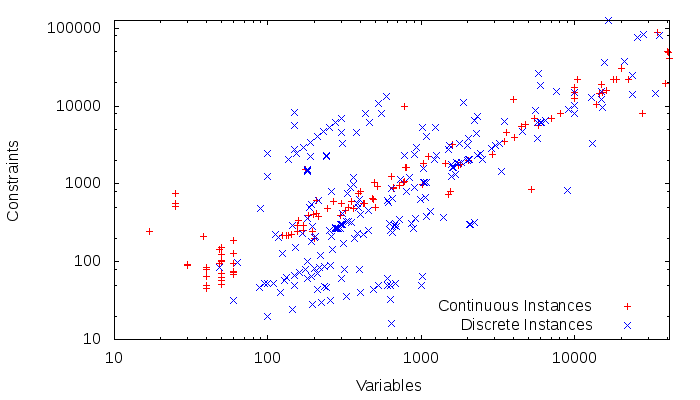
\includegraphics[width=0.85\textwidth]{pic_overview.png}
  \caption{Distribution of variables and constrains  of the qplib
instances \label{fig:1}}
\end{figure}

%%%%%%%%%%%%%%%%%%%%%%%%%%%%%%%
\begin{figure}\centering
  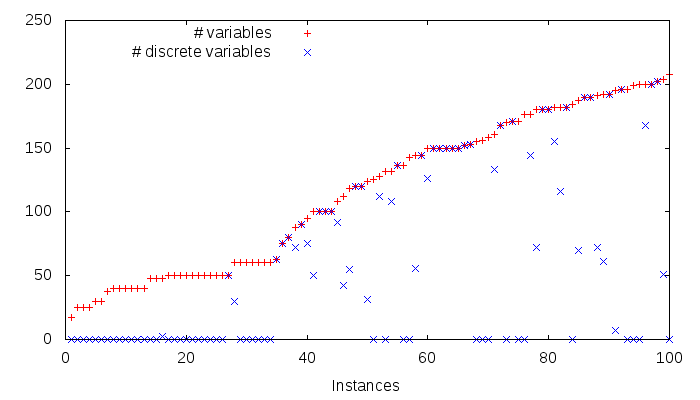
\includegraphics[width=0.85\textwidth]{pic_var_small.png}
  \caption{Number of variables (a) \label{fig:pic_var_small}}
\end{figure}

\begin{figure}\centering
  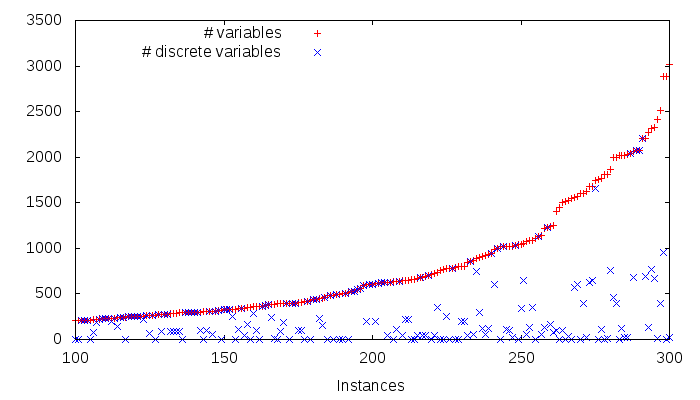
\includegraphics[width=0.85\textwidth]{pic_var_medium.png}
  \caption{Number of variables (b) \label{fig:pic_var_medium}}
\end{figure}

\begin{figure}\centering
  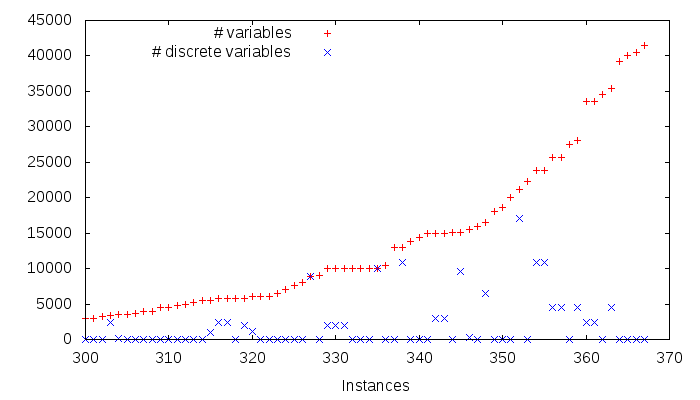
\includegraphics[width=0.85\textwidth]{pic_var_big.png}
  \caption{Number of variables (c) \label{fig:pic_var_large}}
\end{figure}

%%%%%%%%%%%%%%%%%%%%%%%%%%%%%%%%%%%%%%%
\begin{figure}\centering
  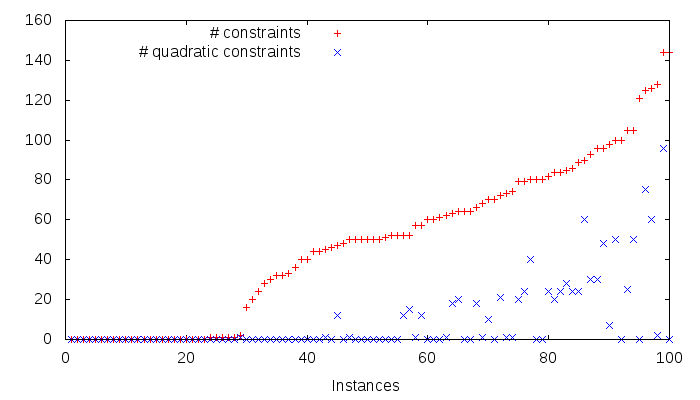
\includegraphics[width=0.85\textwidth]{pic_constr_small.png}
  \caption{Number of constraints (a) \label{fig:pic_constr_small}}
\end{figure}

\begin{figure}\centering
  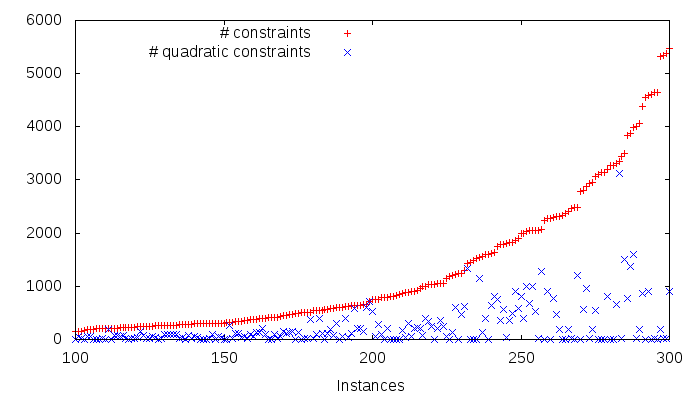
\includegraphics[width=0.85\textwidth]{pic_constr_medium.png}
  \caption{Number of constraints (b) \label{fig:pic_constr_medium}}
\end{figure}

\begin{figure}\centering
  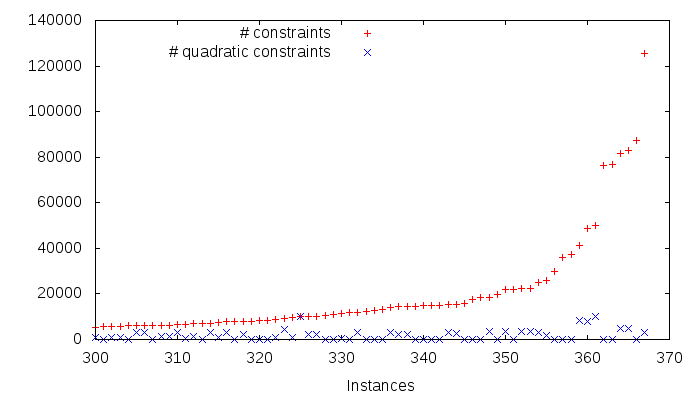
\includegraphics[width=0.85\textwidth]{pic_constr_big.png}
  \caption{Number of constraints (c) \label{fig:pic_constr_big}}
\end{figure}
%%%%%%%%%%%%%%%%%%%%%%%%%%%%%%%%%%%%%%%%%

%\begin{figure}\centering
%  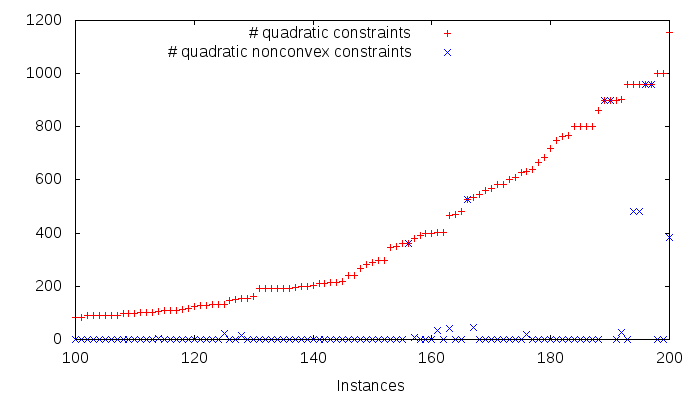
\includegraphics[width=0.85\textwidth]{pic_quad_vs_convex_constr.png}
%  \caption{Number of quadratic constraints (convex and non-convex)
%\label{fig:pic_quad_vs_convex_constr}}
%\end{figure}
%%%%%%%%%%%%%%%%%%%%%%%%%%%%%%%%%%%%%%%%


%\begin{figure}\centering
%  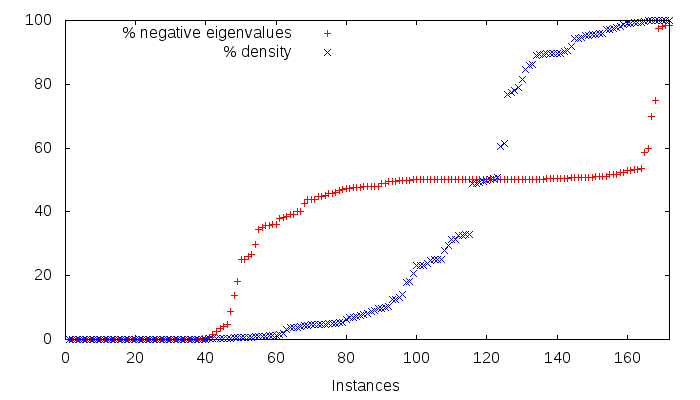
\includegraphics[width=0.85\textwidth]{pic_fuffa.png}
%  \caption{...\label{fig:9}}
%\end{figure}

\begin{figure}\centering
  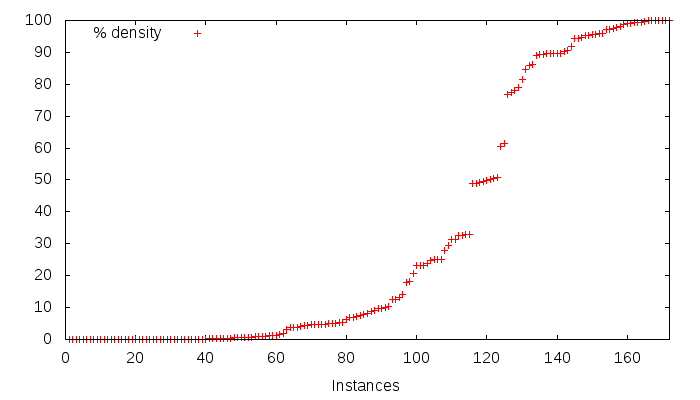
\includegraphics[width=0.85\textwidth]{pic_density.png}
  \caption{Density \label{fig:pic_density}}
\end{figure}

\begin{figure}\centering
  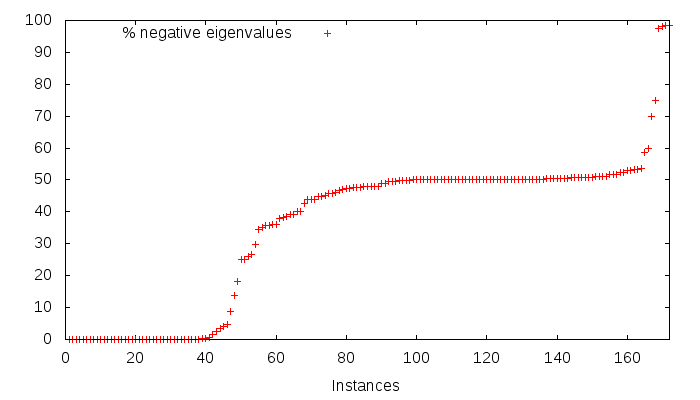
\includegraphics[width=0.85\textwidth]{pic_neg_eig.png}
  \caption{Negative eigenvalues \label{fig:pic_neg_eig}}
\end{figure}









%- - - - - - - - - - - - - - - - - - - - - - - - - - - - - - - - - - - -








%- - - - - - - - - - - - - - - - - - - - - - - - - - - - - - - - - - - -
%- - - - - - - - - - - - - - - - - - - - - - - - - - - - - - - - - - - -
%  End QPLIB-3.tex
%- - - - - - - - - - - - - - - - - - - - - - - - - - - - - - - - - - - -
%- - - - - - - - - - - - - - - - - - - - - - - - - - - - - - - - - - - -
